\begin{surferPage}[七次曲面]{对称七次曲面}
这个像星星一样的曲面是个7次曲面。它的奇异点数84一直以来都是已知最大的奇异点数。直到2004年,奥利弗 莱布斯将最大奇异点数提高到99。
从图中观察到的三个垫子是由车比雪夫多项式导致的,这与奇穆托夫八次曲面类似。实际上,这个星形曲面是奇穆托夫曲面的一个变形。对某个适当选取的$\lambda\in\RR$,这里平面曲线$S_7(xy)$: \[S_7(x,y) + \lambda \cdot T_d(z) = 0,\] $T_d(x)+T_d(y)$ 被一个正7边形所替代。
\vspace*{-0.3em}
    \begin{center}
      \begin{tabular}{c@{\qquad}c}
        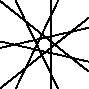
\includegraphics[height=1.5cm]{./../../common/images/labsseptic1.pdf}
        &
        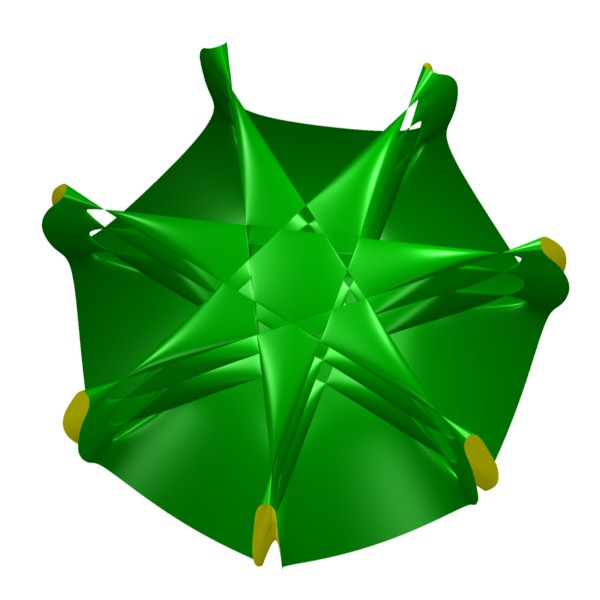
\includegraphics[height=1.5cm]{./../../common/images/septic_7eck_von_oben}
      \end{tabular}
    \end{center}
    \vspace*{-0.3em}
这个奇穆托夫构造的变形是由杜克范斯特拉滕提供的。
\end{surferPage}
